
% This LaTeX was auto-generated from MATLAB code.
% To make changes, update the MATLAB code and republish this document.

\documentclass{article}
\usepackage{graphicx}
\usepackage{color}

\sloppy
\definecolor{lightgray}{gray}{0.5}
\setlength{\parindent}{0pt}

\begin{document}

    
    
\subsection*{Contents}

\begin{itemize}
\setlength{\itemsep}{-1ex}
   \item AMSC 460 - HW11
   \item Problem 1 (finished)(AFFRImative)
   \item Problem 2 (WTh)
\end{itemize}


\subsection*{AMSC 460 - HW11}

\begin{verbatim}
clear all; format compact; close all; syms f(x) x y z
\end{verbatim}


\subsection*{Problem 1 (finished)(AFFRImative)}

\begin{par}
Write down the polynomial that interpolates f(x) = e\^{}x at the points x0 = 0 and x1 = 1 in Lagrange form and Newton form (using divided differences). Check that these polynomials are the same.
\end{par} \vspace{1em}
\begin{par}
f(x) = e\^{}x, so the three points are (0,1) (1,e) P(x)= 1((x-1)/(0-1))+e((x-0)/(1-0)) The final answer is P(x)=ex-x+1
\end{par} \vspace{1em}


\subsection*{Problem 2 (WTh)}

\begin{par}
The Vandermonde matrix can be badly conditioned and is not ideal for solving many interpolation problems. On the other hand, some of this ill-conditioning can be mitigated by scaling the data. Suppose we are given data points (x0, y0), ..,(xn, yn) with x0 \ensuremath{<} x1 \ensuremath{<} ... \ensuremath{<} xn. Consider scaling the x values by letting zi = xi - α/β where α and β are given numbers with β \ensuremath{>} 0. The data points (xi, yi) change to (zi, yi), and the interpolation polynomial changes to pn(z) = a0 + a1z + · · · + anzn.
\end{par} \vspace{1em}
\begin{par}
(a) The original data interval is x0 ≤ x ≤ xn. What is the data interval when using z = (x − α)/β? What matrix equation must be solved to find the a’is in the above formula for pn(z)?
\end{par} \vspace{1em}
\begin{par}
(b) Taking a hint from the previous step, the data will be scaled so that the new data interval is instead −1 ≤ z ≤ 1. What must α and β be here?
\end{par} \vspace{1em}

\begin{verbatim}  Then z0 = (x0-α)/β = -1  => x0 = -β+α
  and  zn = (xn-α)/β = 1   => xn =  β+α
  Then x0 + xn = -β+α+β+α = 2α
       =>      α = (x0 + xn) / 2
  and  xn - x0 = β+α - (-β+α) = 2β
       =>      β = (xn - x0) / 2\end{verbatim}
    \begin{par}
(c) Consider the following population data for the USA over the 100 year period between 1900 and 2000. The y values represent the population of the USA in millions. Using the direct approach (Vandermonde), plot the interpolation function using the original xi data. You should use MATLAB’s vander command to construct the Vandermode matrix V . Using MATLABs cond commmand, what is the condition number cond(V) of the associated Vandermonde matrix V ?
\end{par} \vspace{1em}
\begin{verbatim}
x = [1900 1910 1920 1930 1940 1950 1960 1970 1980 1990 2000];
y = [76.21; 92.23; 106; 123.2; 151.3; 179.3; 203.3; 226.5; 248.8; 281.4; 308.7]*1000000;
V = vander(x)
\end{verbatim}

        \color{lightgray} \begin{verbatim}V =
   1.0e+33 *
  Columns 1 through 7
    0.6131    0.0003    0.0000    0.0000    0.0000    0.0000    0.0000
    0.6462    0.0003    0.0000    0.0000    0.0000    0.0000    0.0000
    0.6808    0.0004    0.0000    0.0000    0.0000    0.0000    0.0000
    0.7171    0.0004    0.0000    0.0000    0.0000    0.0000    0.0000
    0.7551    0.0004    0.0000    0.0000    0.0000    0.0000    0.0000
    0.7950    0.0004    0.0000    0.0000    0.0000    0.0000    0.0000
    0.8367    0.0004    0.0000    0.0000    0.0000    0.0000    0.0000
    0.8804    0.0004    0.0000    0.0000    0.0000    0.0000    0.0000
    0.9261    0.0005    0.0000    0.0000    0.0000    0.0000    0.0000
    0.9739    0.0005    0.0000    0.0000    0.0000    0.0000    0.0000
    1.0240    0.0005    0.0000    0.0000    0.0000    0.0000    0.0000
  Columns 8 through 11
    0.0000    0.0000    0.0000    0.0000
    0.0000    0.0000    0.0000    0.0000
    0.0000    0.0000    0.0000    0.0000
    0.0000    0.0000    0.0000    0.0000
    0.0000    0.0000    0.0000    0.0000
    0.0000    0.0000    0.0000    0.0000
    0.0000    0.0000    0.0000    0.0000
    0.0000    0.0000    0.0000    0.0000
    0.0000    0.0000    0.0000    0.0000
    0.0000    0.0000    0.0000    0.0000
    0.0000    0.0000    0.0000    0.0000
\end{verbatim} \color{black}
    \begin{verbatim}
cond(V)
\end{verbatim}

        \color{lightgray} \begin{verbatim}ans =
   6.5717e+48
\end{verbatim} \color{black}
    \begin{verbatim}
p = V\y;
t = linspace(1900,2000,11);
f = polyval(p,t);
plot(x,y,'o',t,f,'r-+')
legend({'given y', 'estimate y using Vandermonde'})
\end{verbatim}

        \color{lightgray} \begin{verbatim}Warning: Matrix is close to singular or badly scaled. Results may be inaccurate.
RCOND =  2.119618e-49. 
\end{verbatim} \color{black}
    
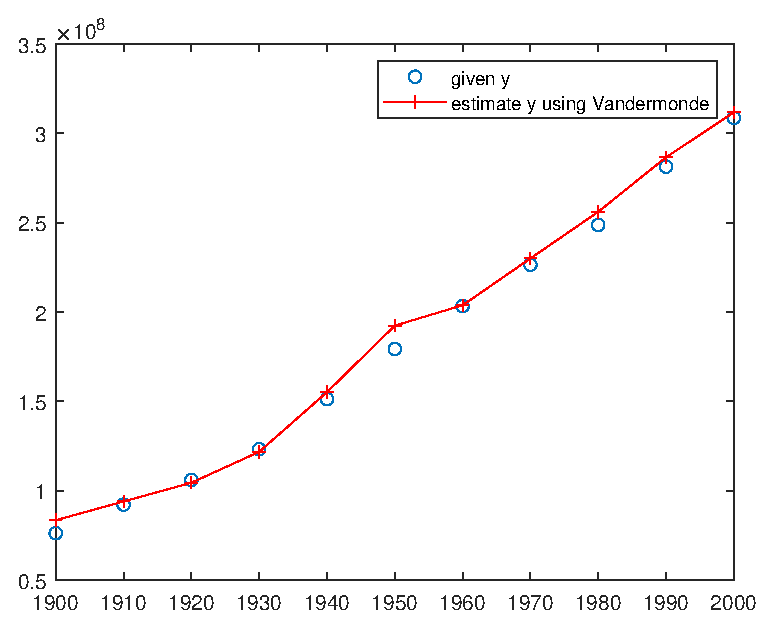
\includegraphics [width=4in]{hw11_01.eps}
\begin{par}
(d) Using the same population data from part (c), scale the data to [−1, 1] and find the coefficients for pn(z). What is the condition number in this case? Once the a'is are computed the resulting (unscaled) polynomial is pn(x) = a0 + a1(x − α/β) + · · ·an(x − α/β)\^{}n.
\end{par} \vspace{1em}
\begin{par}
Plot this function and compare it with the function you found in part (c). Com- ment on the difference between the two.
\end{par} \vspace{1em}
\begin{verbatim}
a = (2000+1900)/2; % α = (x0 + xn) / 2
b = (2000-1900)/2; % β = (xn - x0) / 2
disp('Scale the data to [−1, 1]:')
z = (x-a)/b
\end{verbatim}

        \color{lightgray} \begin{verbatim}Scale the data to [−1, 1]:
z =
  Columns 1 through 7
   -1.0000   -0.8000   -0.6000   -0.4000   -0.2000         0    0.2000
  Columns 8 through 11
    0.4000    0.6000    0.8000    1.0000
\end{verbatim} \color{black}
    
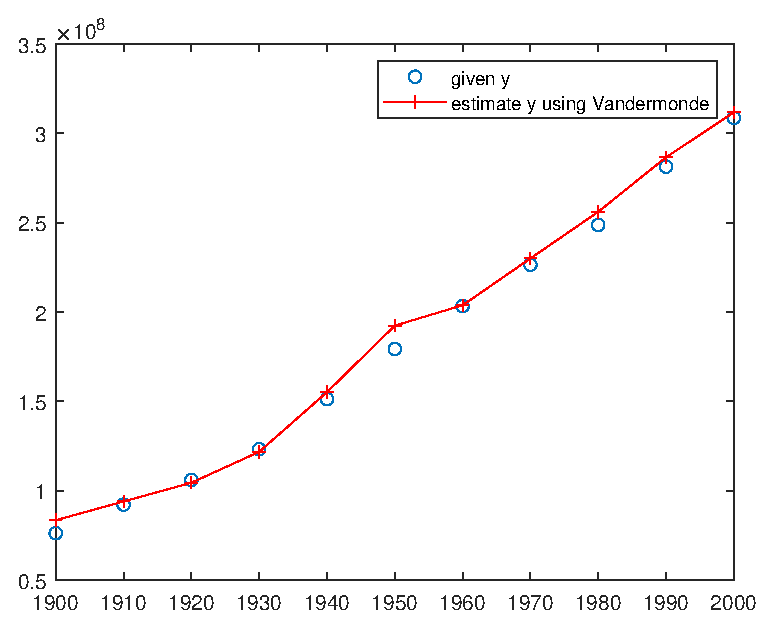
\includegraphics [width=4in]{hw11_02.eps}
\begin{verbatim}
disp('The new Vandermode matrix V:')
Vz = vander(z)
\end{verbatim}

        \color{lightgray} \begin{verbatim}The new Vandermode matrix V:
Vz =
  Columns 1 through 7
    1.0000   -1.0000    1.0000   -1.0000    1.0000   -1.0000    1.0000
    0.1074   -0.1342    0.1678   -0.2097    0.2621   -0.3277    0.4096
    0.0060   -0.0101    0.0168   -0.0280    0.0467   -0.0778    0.1296
    0.0001   -0.0003    0.0007   -0.0016    0.0041   -0.0102    0.0256
    0.0000   -0.0000    0.0000   -0.0000    0.0001   -0.0003    0.0016
         0         0         0         0         0         0         0
    0.0000    0.0000    0.0000    0.0000    0.0001    0.0003    0.0016
    0.0001    0.0003    0.0007    0.0016    0.0041    0.0102    0.0256
    0.0060    0.0101    0.0168    0.0280    0.0467    0.0778    0.1296
    0.1074    0.1342    0.1678    0.2097    0.2621    0.3277    0.4096
    1.0000    1.0000    1.0000    1.0000    1.0000    1.0000    1.0000
  Columns 8 through 11
   -1.0000    1.0000   -1.0000    1.0000
   -0.5120    0.6400   -0.8000    1.0000
   -0.2160    0.3600   -0.6000    1.0000
   -0.0640    0.1600   -0.4000    1.0000
   -0.0080    0.0400   -0.2000    1.0000
         0         0         0    1.0000
    0.0080    0.0400    0.2000    1.0000
    0.0640    0.1600    0.4000    1.0000
    0.2160    0.3600    0.6000    1.0000
    0.5120    0.6400    0.8000    1.0000
    1.0000    1.0000    1.0000    1.0000
\end{verbatim} \color{black}
    \begin{verbatim}
disp('The new condition number:')
cond(Vz)
\end{verbatim}

        \color{lightgray} \begin{verbatim}The new condition number:
ans =
   1.3952e+04
\end{verbatim} \color{black}
    \begin{verbatim}
disp('the coefficients for pn(z):')
p2 = Vz\y
\end{verbatim}

        \color{lightgray} \begin{verbatim}the coefficients for pn(z):
p2 =
   1.0e+09 *
   -0.1803
   -0.5373
    0.4123
    1.0368
   -0.4142
   -0.5896
    0.2549
    0.0787
   -0.0596
    0.1277
    0.1793
\end{verbatim} \color{black}
    \begin{verbatim}
t = linspace(-1,1,11);
f2 = polyval(p2,t);
plot(z,y,'o',t,f2,'g-+')
legend({'given y', 'estimate y using Vandermonde'})
\end{verbatim}

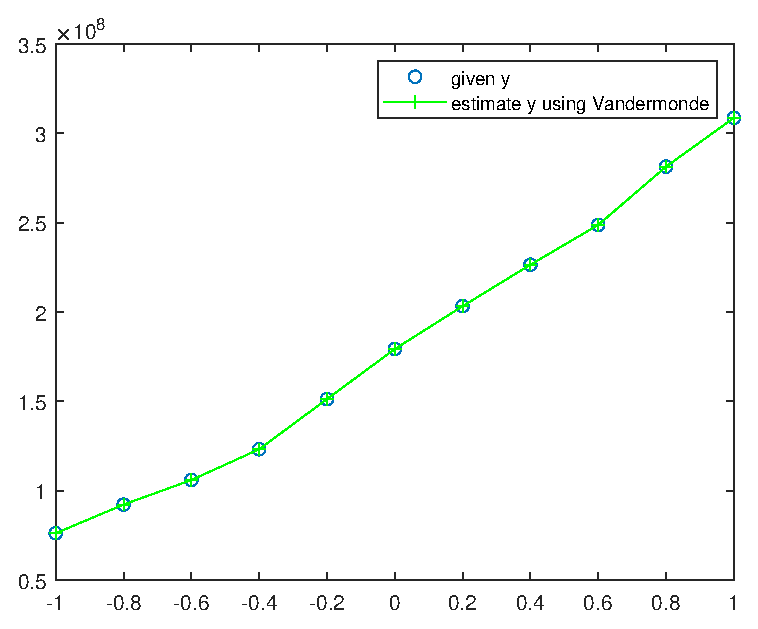
\includegraphics [width=4in]{hw11_03.eps}

\begin{verbatim}  The y using interpolation function in 4(d) is more accurate,
  Also the condition number in 4(d) is way smaller than the condition number in 4(c)\end{verbatim}
    


\end{document}

